\documentclass[crop]{CSLB}

%The authors can define any packages after the \documentclass{CSL} command.
\usepackage{amsmath} %for dealing with mathematics,
\usepackage{amsthm} %for dealing with theorem environments,
\usepackage{cite} %%%for dealing with citations
\usepackage{hyperref} %for linking the cross references
\usepackage{graphics} %for dealing with figures.
\usepackage{algorithmic} %for describing algorithms
\usepackage{subfig} %for getting the subfigures e.g., "Figure 1a and 1b" etc.
\usepackage{url} %It provides better support for handling and breaking URLs.

%\usepackage{natbib}
\usepackage{boites}

%\usepackage{graphicx}
%\usepackage{float}
%\usepackage{psfig}
%\usepackage{amsfonts,amssymb}
%\usepackage{color}
%\usepackage{textcomp}
%\usepackage[T1]{fontenc}
%\usepackage{aecompl}
%\usepackage{times}
%\usepackage{txfonts}
%\usepackage[english]{babel}
%\usepackage[utf8x]{inputenc}
%\usepackage{amsmath}
%\usepackage{caption}
%\usepackage{siunitx} 

\jname{International Journal of Astrobiology}%

\newtheorem{theorem}{Theorem}
\newtheorem{condition}{Condition}
 
\newcommand{\ceti}{CCN}
\newcommand{\cetis}{CCNs}
\newcommand{\hs}{\textsc{hearsay}}

\newcommand{\awakening}{A event }
\newcommand{\contact}{C event }
\newcommand{\blackout}{B event }
\newcommand{\doomsday}{D event }

\newcommand{\aawakening}{Awakening event }
\newcommand{\ccontact}{Contact event }
\newcommand{\bblackout}{Blackout event }
\newcommand{\ddoomsday}{Doomsday event }

\newcommand{\awakenings}{A events }
\newcommand{\contacts}{C events }
\newcommand{\blackouts}{B events }
\newcommand{\doomsdays}{D events }

\newcommand{\ff}{{\color{red}\rule{10pt}{10pt}}}

%\newcommand{\ffn}[1]{ \colorbox{red}{FIG {#1}} }    
\newcommand{\ffn}[1]{}

%\newcommand{\ttn}[1]{ \colorbox{green}{TABLE {#1}} }    
\newcommand{\ttn}[1]{}



\begin{document}

\supertitle{Research Paper}

\title[Probabilities of SETI contacts]{Probability of causal
contact between interstellar civilizations through MonteCarlo simulations}

\author[Lares, Funes \& Gramajo]{Lares M.$^{1, 2}$, Funes J.~G.$^{1,
3}$ \& Gramajo L.$^{1, 2}$}

\corres{\name{Lares M} \email{marcelo.lares@unc.edu.ar}}

\address{
   \add{1}{CONICET, Argentina}

   \add{2}{Universidad Nacional de C\'ordoba, Observatorio
           Astron\'omico de C\'ordoba, Argentina}

   \add{3}{Universidad Cat\'olica de C\'ordoba, Argentina}
}
 

\keywords{SETI, Computer simulations, Statistics}

%\JELclassification{XX; XX}
%\MSCcodes{XX; XX}

\Abbreviations{SETI: Search for Extraterrestrial Intelligence,\\
CCN: causally connected node,\\
SFC: surface of first contact,\\
SLC: surface of last contact,\\
DE: Discrete Event,\\
GHZ: Galactic Habitable Zone}
 

\begin{abstract}
%
The abundance of intelligent civilizations in the Galaxy is a
   longstanding question, often conceptualized as the problem of the
   lack of received communication. Estimates of the number of
   civilizations are generally guided by the Drake equation, despite
   the large uncertainties in its factors and its lack of a temporal
   nature. Alternative approaches use detailed numerical simulations
   of the galaxy and recipes for the stars and planets formation
   rates and for the origin of life, and rely on uncertain parameters.
   We present a statistical model for the abundance and duration of
   civilizations implemented through Monte Carlo simulations. We
   explore the hypothesis space of the model by a suite of simulations
   to analyze the emergence of communicating nodes and their causal
   connections. We based this on minimal assumptions and three free
   parameters, with focus on the proposed statistical properties of
   empirical models. Our analysis of the dependence of the rate of
   causal contacts on the mean number of civilizations, the mean
   lifespan distribution and the maximum distance a civilization can
   send signals, is considered to discuss the spatial and temporal
   structure of a populated galaxy within several scenarios. We find
   that, given the enormous distances involved, causal contacts
   between civilizations are very rare. The odds to make a contact in
   a few years of monitoring are low for most models, except for those
   of a galaxy densely populated with long-lived civilizations. The
   probability of causal contacts increases with the lifetime of
   civilizations much more significantly than with the number of
   active civilizations for a time window. We show that the maximum
   probability of making a contact occurs when a civilization gains
   the required communication technology.
%
\end{abstract}

\maketitle


%%% S E C T I O N - - - - - - - - - - - - - - - - - - - - - - -
\section{Motivations}\label{S_motivations}
%{{{

The Drake equation  \citep{drake_intelligent_1962} provides a truly
helpful educated guess, a rational set of lenses –the factors in the
equation– through which to look at future contacts with
technologically advanced civilizations in the Milky Way. 
%
The equation quantifies the number of civilizations from whom we might
receive an electromagnetic signal, using a collection of factors that
have been extensively discussed in the literature and whose estimates
are revised continually. 
%
A comprehensive review and analysis of each term of the equation are
presented in \citet{vakoch_drake_2015}.
%
Optimistic estimates from the Drake equation contrast with the
so-called Fermi paradox, which states the contradiction between the
expected abundance of life in the Galaxy and the lack of evidence for
it \citep[e.g. ][]{hart_explanation_1975, brin_great_1983,
barlow_galactic_2012, forgan_galactic_2016, vanhouten_isthere_2017,
Sotos_biotechnology_2019, carroll_nellemback_fermi_2019}.
%
There are many propositions aimed at solving this paradox, which make
use of statistical \citep{solomonides_probabilistic_2016,
vanhouten_isthere_2017, horvat_calculating_2007,
maccone_statistical_2015} or stochastic approaches
\citep{forgan_numerical_2009, bloetscher_using_2019,
glade_stochastic_2011, forgan_numerical_2010}.
%
Regarding the Drake equation, analytical interpretations
\citep{prantzos_joint_2013, smith_broadcasting_2009} or reformulations
\citep[][and references therein]{burchell_whither_2006} have also been
proposed. 
%
The lack of contacts could be explained by the difficulty of life to
appear due to astrophysical explanations
\citep{annis_astrophysical_1999}.
%
In general, also more speculative proposals
\citep{barlow_galactic_2013, lampton_information_2013,
conway_three_2018, forgan_galactic_2017} have been discussed.
% 
% 
% 
% 
\Fpagebreak
%
We stress the fact that the only observation that can be stated with
certainty is that for the number of years projects for the Search of
Extraterrestrial Intelligences (SETI) have been working; we have
received no signal using the technical possibilities and the
conditions established by them \citep{tarter_search_2001}.
%
The absence of detection has also motivated alternative ideas for new
SETI strategies \citep{forgan_exoplanet_2017, balbi_impact_2018,
loeb_eavesdropping_2006, maccone_KLT_2010, tarter_advancing_2009,
enriquez_breakthrough_2017, loeb_relative_2016, maccone_SETI_2011,
lingam_relative_2019, wright_theGsearch_2015, maccone_SETI_2013,
maccone_lognormals_2014, harp_application_2018,
forgan_possibility_2013, forgan_galactic_2017, funes_searching_2019}.
%
The Drake equation is a key tool to organise the discussion about the
problem of the (unknown) abundance of civilisations in the Galaxy
\citep{hinkel_interdisciplinary_2019}.
%
However, the uncertainties in the factors of this equation make it
less prone to a formal study to define searching strategies or to
compute the actual number of extraterrestrial intelligences.
%
The optimistic estimations from the Drake equation also contrast with
the SETI initiatives, noticeable overshadowed because despite decades
of effort, not a single evidence for intelligent signals has been
detected.
%
\citet{prantzos_joint_2013} proposes a unified framework for a joint
analysis of the Drake equation and the Fermi paradox, concluding that
for sufficiently long-lived civilisations, colonisation of the Galaxy
is the only reasonable option to gain awareness about other life
forms.
%
\citet{haqq-misra_drake_2017} discuss the dependence of the Drake
equation parameters on the spectral type of the host stars and the
time since the Galaxy formed and examine trajectories for the
emergence of communicative civilisations.
%
Some modifications to the original idea of the equation have tried to
imprint a stochastic nature, to propose a probabilistic approach, or
to consider the temporal structure missing in the equation.
%
Temporal aspects of the distribution of communicating civilisations
and their contacts have also been explored by several authors
\citep{fogg_temporal_1987, forgan_spatiotemporal_2011,
balbi_impact_2018, balb_spatiotemporal_2018, horvat_impact_2011}, as
well as efforts on considering the stochastic nature of the Drake
equation \citep{glade_stochastic_2011}.
%
The literature about this topic brings a number of works that consider
numerical simulations \citep{forgan_evaluating_2015,
vukotic_grandeur_2016, murante_simulating_2015, forgan_numerical_2009,
forgan_galactic_2017, ramirez_new_2017}.
%
Although this approach does not rely on observed quantities that could
be modified with time, it also depend on the definition of a number of
parameters which are unknown or uncertain.
%
\citet{grimaldi_signal_2017} consider a statistical model for the
probability of the Earth contacting other intelligent civilisations,
taking into account the finite lifetime of signal emitters, and based
on the fractional volume occupied by all signals reaching our planet.






In a recent work, \citep{balbi_impact_2018} use a statistical model to
analyse the occurrence of causal contacts between civilisations in the
Galaxy.
%
The author highlights the effect of evolutionary processes when
attempting to estimate the number of communicating civilisations that
might be in causal contact with an observer on the Earth.
%
\citet{cirkovic_temporal_2004} also emphasise the lack of temporal
structure in the Drake equation.
%
\citet{bloetscher_using_2019} uses a probabilistic approach, though
still motivated by the Drake equation, to obtain a probabilistic
measure for the number of civilisations in the Galaxy.
%
To that end, the authors do Monte-Carlo Markov Chains over each factor
of the Drake equation, and combine the means to reach a probabilistic
result.
%
It is worth mentioning that the author proposes a log-normal target
distribution to compute the posterior probabilities.
%
This study concludes that there is a tiny probability for Earth to
contact another extraterrestrial civilization.    
%
\citet{smith_broadcasting_2009} uses an analytical model to gauge the
probabilities of contact between two randomly located civilisations,
and the waiting time for the first contact, assuming a fixed maximum
broadcasting distance.
% 
Adopting a novel approach, \citet{balbi_impact_2018} investigate the
chance of communicating civilisations making causal contact within a
volume surrounding the location of the Earth, using a statistical
model to compute the occurrence of causal contacts.
%
The author stresses the fact that the causal contact requirement
involves the distance between civilisations, their lifespan and their
times of appearance. This is important since the time it takes the
light to travel across the Galaxy is much lesser than its lifetime.
%
\citet{balbi_impact_2018} fix the total number of civilisations and
explore the parameter space that comprise three parameters, namely,
the distance to the Earth, the time of appearance and the lifespan of
the communicating civilization.
%
Each of these three variables are drawn from a random distribution.
The distribution of the distances results from a uniform distribution
of civilizations within the plane of the Galaxy.
%
For the distribution of the characteristic time of appearance, the
author explores an exponential and a truncated Gaussian distributions.
For the distribution of the lifespans, the author chooses an
exponential distribution.
%
\citet{balbi_impact_2018} finds that the fraction of communicating
civilisations vary with the choice of the statistical distribution for
the time of appearance. 
%
For all analysed distributions, the fraction corresponding to a mean
lifetime of 10$^9$ years and for a maximum radius for the detection of
the signal of 1000 yr, is roughly 0.1.
%
In another related approach, \citet{vukotic_astrobiological_2012}
propose a probabilistic cellular automata (PCA) modelling. 
%
In this framework, a complex system is modelled by a lattice of cells
which evolve at discrete time steps, according to transition rules
that take into account for each cell the states of its neighbour
cells.
%
The authors implement a PCA model to a network of cells which
represent life complexity on a 2-dimensional region resembling the
Galactic Habitable Zone (GHZ),  an annular ring set between a minimal
radius of 6 kpc and a peak radius of 10 kpc. 
%
Within this framework, \citet{vukotic_astrobiological_2012} also make
several Monte Carlo simulations and analyse ensemble-averaged results.
%
The work aims at analysing the evolution of life, although it does not
account for the network of causal contacts among
technological civilisations.


In this work we address the problem of the temporal and spatial
structure of the distribution of communicating civilisations.
%
To that end, we reduce and explore the hypothesis space over a set of
three of parameters.
%
We propose to avoid the frequentist approach of the Drake equation to
compute the number of civilisations, providing its statistical
distribution instead.
%
This is an exploratory analysis that aims at providing a numerical
tool to discuss the different scenarios based on statistical
heuristics.
%
With this, we aim at avoiding the several theoretical problems
summarised by the Drake equation factors.
%
The approach proposed here should be considered as a compromise
between the uncertainties of the frequentist approach and the detailed
recipes required on the simulation approach.
%
We provide a framework to explore, through a suite of
numerical simulations, a parameter space of three unknown observables.
%
This allows to discuss possible scenarios and their consequences in
terms of the probability of making contacts.
%
The method we use for simulating a stochastic process is an
approximation that allows to study the behaviour of complex systems,
by considering a sequence of well defined discrete events.
%
The simulation is carried out by following all the variables that
describe and constitute the state of the system, and the evolution of
the process is described as a set of changes in that state.
%
In this context, an event produces a specific change in the state that
can be triggered by random variables that encode the stochastic nature
of the physical phenomenon.
%
For example, when a new contact is produced between two entities in
the simulated galaxy, the numbers of active communication lines and of
communicated nodes does change.
%
The process involves following the changes on the state of the system,
defining the initial and final states.
%
This is done by defining a method that allows to keep track of the
time progress in steps, and maintaining a list of relevant events.
%
In Sec.~\ref{S_methods} we introduce the methods and discuss the
candidate distributions for the statistical aspects of the times
involved in the communication process.
%
We present our results in Sec~\ref{S_results}, with special emphasis
on the statistical distributions of the duration of causal contacts in
one or both directions and the distribution of time intervals for the
waiting of the first contact.
%
This quantities are considered as a function of the three simulation
parameters.
%
In Sec.~\ref{S_discussion} we discuss our results and future research
directions.   
%}}}


%%% S E C T I O N - - - - - - - - - - - - - - - - - - - - - - -
\section{Methods and working hypotheses}\label{S_methods}
%{{{

Simulations are suitable tools to analyse systems that evolve with time and involve randomness.
%
An advantage of a numerical approach is that usually require fewer assumptions and simplifications, and can be applied to systems where analytical models are not easily found.
%
In particular, a suitable tool to model complex stochastic processes through the changes in the state of a system is the discrete--event (hereafter, DE) simulation approach.
%
A system described with the DE paradigm is characterised by a set of actors and events.
%
Actors interact causally through a series of events on a timeline and process them in chronological order \citep{ptolemaeus_system_2014, chung_simulation_2003, ross_simulation_2012}.
%
Each event modify the variables that define the process, producing the corresponding change in the state of the simulated system.
%
This method is well suited for the particular case of the diffusion of intelligent signals in the galaxy and allows to explore several models easily.
%
We simulate the statistical properties of a set of points in space and time that have a causal connection at light speed, dubbed ‘’Causal Contact Nodes’’ (hereafter, \ceti{}).
%
We chose this generic name in order to stress the fact that in this analysis 
only the causal contact is considered, independently of any broadcasting or lookout activity.
%
The system we propose is ideal, in the sense that it considers the special case of a fully efficient node that emits and receives isotropically.
%
A causal contact node, considered as a broadcasting station that has the ability to detect signals through an active lookout program, could have a lesser than one efficiency factor, which is not included in the current analysis.
%
Also, it is worth mentioning that this is a general approach, and not necessarily a \ceti{} is the host of an intelligent civilization.
%
For instance, it can be associated with a planet where life has developed, became intelligent, reached the skills required to find the right communication channel, sustain a search and establish a contact.
%
Alternative message processing entities could be considered, for example interstellar beacons where life has ceased to exist but continue with its emission, or communication stations established by probes or left by intelligent beings \citep[see, e.g., ][]{peters_outer_2018, barlow_galactic_2013}.
%
In principle, these strategies could affect our results since it would be easier to configure a cluster of \cetis{} that spread in time.
%
However, we do not consider these speculative alternatives at this point.
%
For the purpose of the present analysis, only the communication capability is relevant, since we study the causal contacts between the locations.
%
The system is defined by a number of actors that represent \cetis{} and appear at different instants in time, generating events that produce meaningful changes in the variables that describe the system, i.e., in the arrangement of \cetis{} and their network of causal contacts.
%
For example, the appearance of a new \ceti{} in a region filled with a signal emitted by another node, will increase the number of active \cetis{} and the number of pairs of \cetis{} in causal contact.
%
Assuming some simple hypotheses, the discrete events method can be performed taking into account a small number of variables, which allow to analyze the variation of the results in the model parameter space.



In what follows, we outline the experimental setup adopted to estimate the probabilities of causal contacts and several derived quantities.
%
This is done in terms of three independent parameters, namely, the
mean time span between the appearance of consecutive \cetis{},
$\left<\tau_a\right>$, their mean lifetime $\left<\tau_s\right>$, and
the maximum distance a signal can be detected by another \ceti{}
($D_{\rm max}$).
%
Intuitively, the probability of the existence of causal contacts
between pairs of \cetis{} would be larger for smaller $\tau_a$
parameters, higher $\tau_s$ or higher $D_{\rm max}$ parameter values.
%
We also propose theoretical distribution functions for both the lifespans ($\tau_s$) and the number of \cetis{} per unit time \citep{maccone_evolution_2014, Sotos_biotechnology_2019}.
%
The later is related to the time span between the appearance of consecutive \cetis{} (since when $\left<\tau_a\right>$ is shorter, it produces a greater density of \cetis{}).
%
The analytical expresiones for these distributions are set to a fixed law, as discussed in Sec.~\ref{SS_PDF_shape}.  
    
%}}}

\begin{figure}[!t]
   \centering
   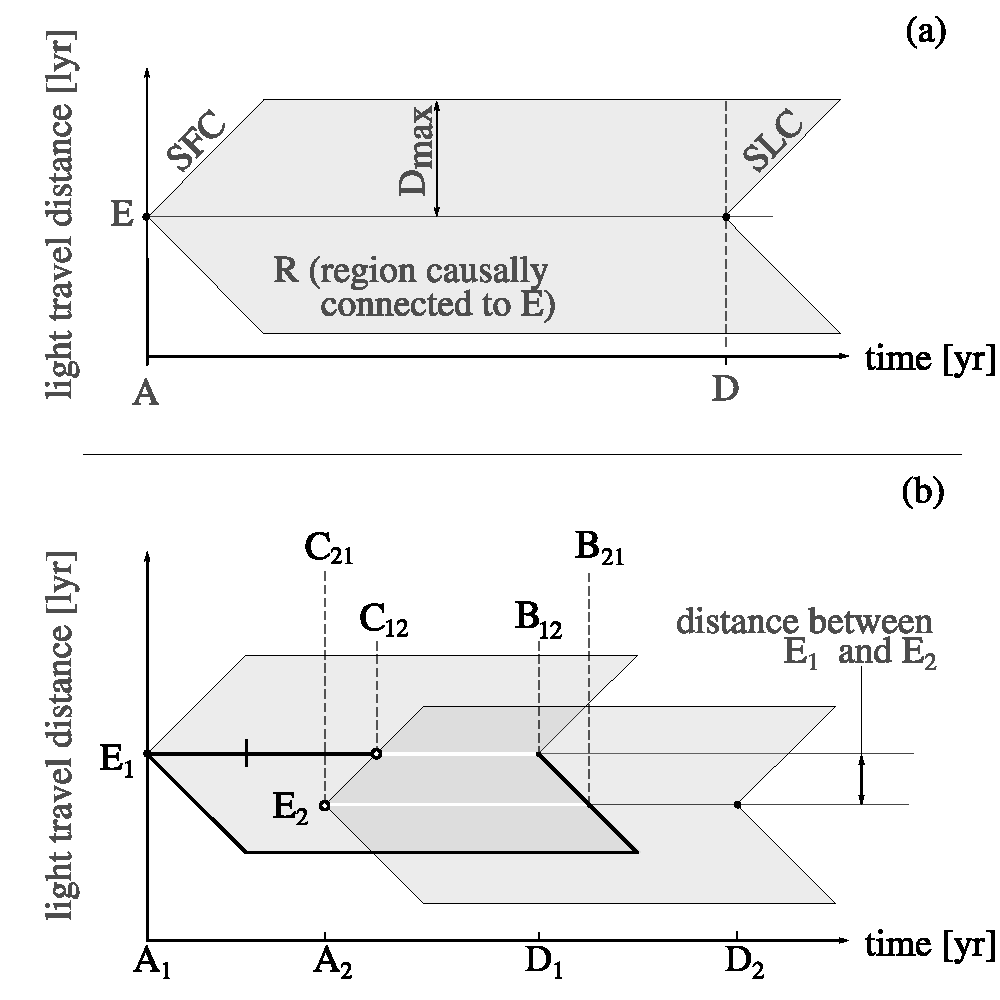
\includegraphics[width=0.5\textwidth]{F_scheme.pdf}
   \caption{
   %
Space--time diagrams showing a schematic representation of the
different stages in the development of causal contact node (\ceti{}).
%
Panel (a) represents the region $R$ in space and time which is causally
connected to the emitter (left vertex), following an "A" type event
("Awakening") in which the node acquires the communication capability.
%
The sphere of first contact (SFC) is a sphere centered on the emitter
that grows until its radius reaches the D$_{\rm max}$ distance, in which
the power of a signal would equal the detectability threshold.
%
In the Figure this sphere is represented by the left triangle of the
region $R$.
%
The surface of last contact (SLC) is another sphere that grows from a
"D" event ("Doomsday").
%
The region which is causally connected to the emitter is then limited
by these two spheres, and has the shape of a sphere or of a spherical
shell, depending on the time.
%
The temporal intervals for
the communication between two \cetis{} are represented in he
panel (b).
%
The receiver \ceti{} E$_1$ can listen signals from the emiter \ceti{} E$_2$,
from the "Contact" event (t=C$_{12}$) up to the "Blackout" event (t=B$_{12}$).
%
Similarly, 
the receiver \ceti{} E$_2$ can listen signals from the emiter \ceti{} E$_1$,
from t=C$_{21}$ up to t=B$_{21}$. 
%
   } \label{F_scheme}
\end{figure}



%{{{   

\ffn{1} Space—time diagrams, where time and space are represented on
the horizontal and vertical axes, respectively, are suitable tools to
describe the causal connections among different nodes.
%
We illustrate in the Fig.~\ref{F_scheme} the schematic representation
of the region causally connected to a given \ceti{}.
%
For the sake of simplicity, we show in the plot the light travel
distance, i.e., the distance traversed by any signal spreading from
the emitter at light speed (for example, any electromagnetic signal).
%
In this scheme, a light pulse would follow a trajectory represented by
a line at 45 degrees from the axes, given the units of the time and
space axes are years and light years, respectively.
%
Panel (a) of the Figure represents the region $R$ (shaded polygon)
which is causally connected to the emitter (left vertex).
%
This region develops after an event (hereafter dubbed A-type event) in
which the node acquires the communication capability, or becomes
''active''.
%
The sphere of first contact (SFC) is centred on the emitter,
represented in the Figure by the left angle of the region $R$.
%
This sphere grows until its radius reaches the D$_{\rm max}$ distance, in
which it would be no longer detectable due to the decrease in the
energy per unit area, which falls under the assumed detectability
threshold.
%
Similarly, the surface of last contact (SLC) is another sphere that
grows from an event in which the nodes ceases to possess the
communication capability (D type event), and carries the last signal
produced by the emitter.
%
The region which is causally connected to the emitter is then limited
by these two spheres and therefore has the shape of a filled sphere
(before the D event) or of a spherical shell (after the D event).
%
The temporal intervals for the communication between two \cetis{} are
represented in the panel (b) of the Figure.
%
In this scheme, the entire lifetime of a \ceti{} can be represented by
a polygon, as shown in the Figure.
%
The polygon is limited in the spatial axis by the maximum distance of
the signal $D_{\rm max}$ and in the time axis by the time span between the
A-type event (concave vertex) and the D-type event (convex vertex).
%
This representation allows to visualize the important events that
result from the presence and communications of two \cetis{}.
%
The points in time where the \cetis{} acquire their communicating
capacity are dubbed ‘’Awakening’’ events ($A_1$ and $A_2$ in the
Figure).
%
Similarly, the instants in time where the \cetis{} lose their
communicating capacity are dubbed ‘’Doomsday’’ events ($D_1$ and $D_2$
in the Figure).
%
The points in space--time where the first contact is produced for each
one of the \cetis{}, are defined as ''Contact'' events, shown as $C_1$
and $C_2$.
%
Finally, the two points where the contact is lost for each one the
\cetis{}, are denominated ''Blackout'' events, presented as $B_1$ and
$B_2$ in the Figure.
%
The receiver node E$_1$ can listen signals from the emitter node
E$_2$, from the first contact event (t=C$_{12}$) until the last
one (t=B$_{12}$).
%
Similarly, the receiver node E$_2$ can listen signals from the emitter
node E$_1$, from t=C$_{21}$ up to t=B$_{21}$.
%
The time intervals for the open communication channel are determined
by the ''C'' and ''B'' type events.
%
It is noteworthy the fact that there is a time delay between the
contact events of the two \cetis{} involved in this analysis, and also
a time delay between the two blackout events.
%
Therefore, the time range when a bidirectional contact is possible
occurs between the maximum time of the contact points and the minimum
time between the blackout points.

%}}} 
      
  
\begin{figure*}
   \centering
   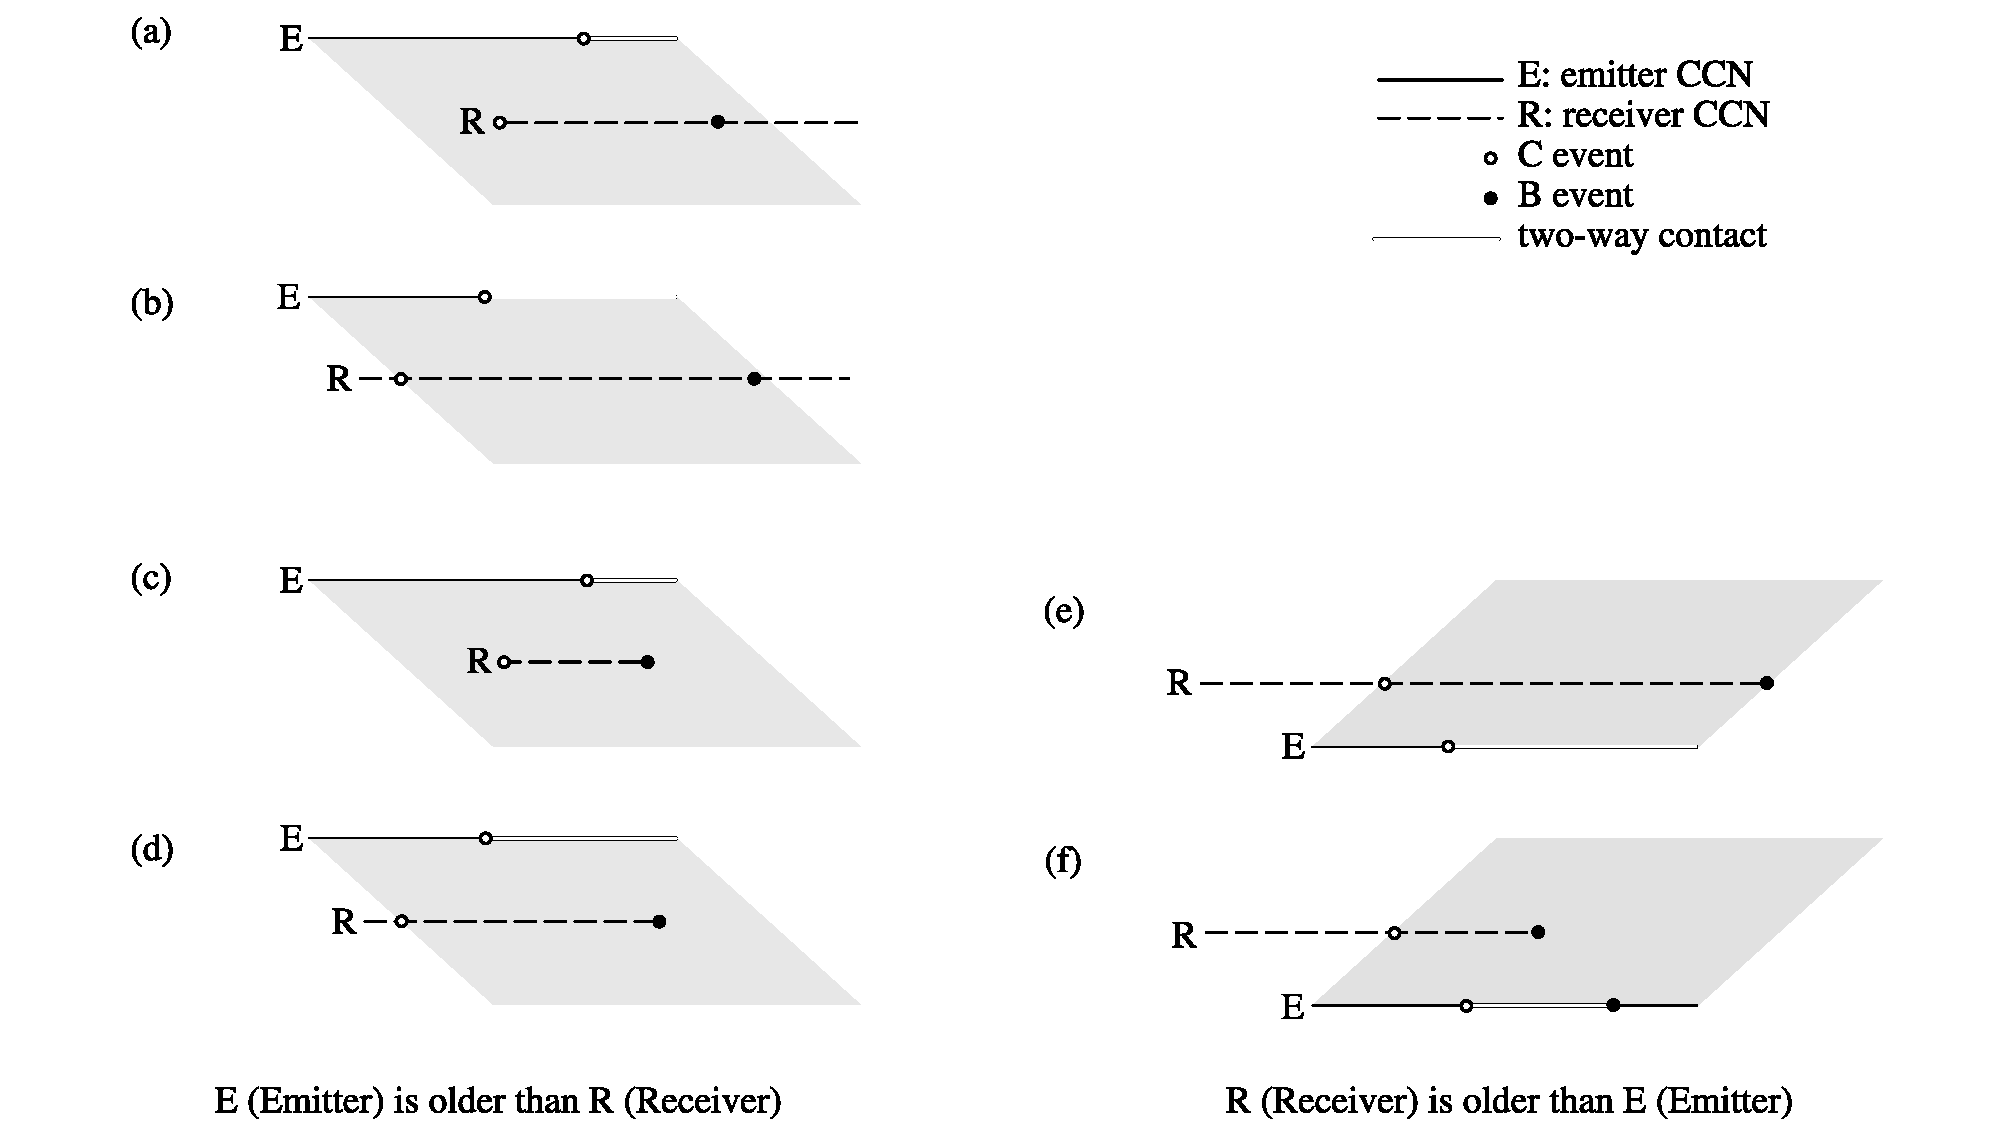
\includegraphics[width=\textwidth]{F_messages.pdf}
   \caption{
   %   
Schematic representation on space--time diagrams of the possible cases in which a
\ceti{} E (Emiter, solid line) can be in causal contact with a \ceti{} R
(Receiver, dashed line).
%
Causal contact can be produced either if the emiter \ceti{} appears before
(left) or after (right) the receiver \ceti{}.
%
The causal contact in which the receiver can have access to the signal 
from the emiter is produced between the C event (Contact, open circles) and the B
event (Blackout, filled circles).
%
The duration of the causal contact in one direction depends on
several factors, mainly the time lag between the awakening events
(horizontal separation in the space--time diagrams)
and the distance between the \cetis (vertical separation in the
space--time diagrams).
%   
The different configurations must be taken into account in order to 
obtain the list of the upcomming events.
%
The time intervals for a two--way communication to be possible are
indicated in double lines. 
%
   } \label{F_messages}
\end{figure*}  


%{{{     

The temporal structure that emerges from the experimental setup implies that, as a fundamental property of the simulations, a causal connection can be produced without 
requiring that the two nodes are active at the same time.
%
This property of the system arises as a consequence of the large spatial and temporal scales, where a message is transmitted at the (relatively small) light speed.
%
Although a \ceti{} could be active for a large enough period to transmit a message at large distances, the limited power of the message and the dilution that depends on the squared distance from the source imposes a detectability limit.
%
As a consequence of this limitation and of their finite lifetime, considered as the period between the acquisition and loss of communicating capacity, each \ceti{} will fill a spherical shell region of the galaxy, limited by two concentric spherical surfaces.
%
The leading front, or surface of first contact (SFC) grows from the
central \ceti{} until it reaches the maximum distance $D_{\rm max}$.
%
Following the end of the civilization, there is still a region which is filled with the emitted signals.
%
This approach has been also considered in other statistical models \citep[e.g., ][]{smith_broadcasting_2009, grimaldi_signal_2017, Grimaldi2018}.
%
The trailing front, or surface of last contact (SLC) also grows from the central \ceti{}, with a delay with respect to the SFC equivalent to the lifetime of the node, and produces a spherical shell region.
%
Any other \ceti{} within this region will be aware of the originating node, even if it has disappeared before the time of contact.
%
This region will grow if the surface of first contact has not yet
reached the maximum distance $D_{\rm max}$, and will shrink after a
D-type event until the surface of last contact reaches $D_{\rm max}$, producing as a result the loss of all signal from the central \ceti{}.
%
In our approach, we consider a model galaxy where the width of the disk is negligible with respect to the radius of the disk.
%
In the 2D simulation only the intersection of the communicating spherical shells with the plane of the galaxy is relevant, and produce the corresponding circles or rings for the filled spheres or annular regions of the spherical shells, respectively.
%
The initially growing communicating sphere is shown over space--time diagrams, where time is represented on the horizontal direction, and space is represented in the vertical direction.
%
In the Fig.~\ref{F_scheme} the two emitters in panel (b), E$_1$ and E$_2$, reach each other at different times.
%
The time span for E$_i$ is (A$_i$ , D$_i$) , for $i = {1, 2}$.
%
Emitter $i$ can listen to emiter $j$ between C$_{ij}$ and B$_{ij}$.
%
The type and length of causal contact in both directions depend on the distance and time lag between the awakening events, the maximum distance that a signal can reach and the time period in which each emitter is active.
%
\ffn{2}
%
In the Fig.~\ref{F_messages} we show a schematic representation of the possible cases in which a \ceti{} E (standing for Emiter) can be in causal contact with a \ceti{} R (receiver).
%
The duration of such a contact in one way depends on several factors, mainly the lifetimes, the time delay between the A-type events and the distance between the two nodes.
%
As it can be seen, the direction of the causal contact does not imply any ordering for the A-type events of the involved emitter/receiver pair.
%
For instance, a node can be in the light cone of another node that turned up later, i.e., the receiver is older than the emitter, like in the cases (e) and (f) of the Figure.
%
In the implementation of the DE simulation, all possibilities for causal contacts are reduced to the six cases shown in the Figure.
%
Once a pair of nodes become active and their properties have been assigned, it is possible to determine if and when they will get connected.
%
The times derived for such events are added to a stack of times so that they are visited in order, and in turn trigger further events.
%
% EJEMPLOS???



In our experimental configuration the simulation starts assuming the stochastic process is already stable, and finishes before any galactic evolution effect could modify the fixed values of the variables.
%
Likewise, we assume that the probability for the appearance of a \ceti{} is homogeneous over the GHZ.
%
Although the Galaxy has a well-known spiral structure, the assumed sparsity of nodes (arguably, intelligent civilisations) does make that assumption tenable.
%
If the distribution of nodes is not sparse, as it could be the case if the spiral arms host most of the \cetis{}, then contacts would be more frequent between closely located nodes.
%
In such a case our results would underestimate the number of contacts between close pairs of nodes within the same spiral arm, and conversely, overestimate the number of contacts between separated nodes.
%
We also limit the possibilities of life or other types of civilisations to the usually stated hypothesis for the definition of
the GHZ \citep{dayal_habitability_2016, gonzalez_galactic_2001, lineweaver_galactic_2004, gonzalez_habitable_2005,
morrison_extending_2015, haqq-misra_evolution_2019, rahvar_cosmic_2016, gobat_evolution_2016, rahvar_cosmic_2016} and consider that habitability remains constant over time \citep[see, however, ][]{gonzalez_habitable_2005, dayal_habitability_2016, gobat_evolution_2016}.
%
For example, \citet{vukotic_astrobiological_2012} propose
probabilistic cellular automata model to explain the astrobiological
history of the Milky Way. % <<<< FEO
%
This means that we set aside civilisations that could survive in severe conditions or unstable systems, which would prevent the appearance of life as we know it.  



We need to raise the scope of our results by stressing the fact that we are considering causal contacts instead of actual contacts.
%
By a causal contact we mean a configuration, in space and time, in which a node belongs to the light cone of another node.
%
This means that a causal contact does not need to be tied to any actual message emission or detection.
%
In more realistic scenarios, there are several sources of ‘’signal loss’’ with respect to the ideal case.
%
Among them, we can mention temporal and signal power aspects and direction dependent communication capabilties.
%
The results must then be interpreted as the case of ideal nodes, with a perfect efficiency in the emision and reception of signals.
%
The probabilities of contacts presented here are then upper limits to the number of communications between civilization s in the Galaxy, given the implemented hipotheses in the model.
%
The use of light cones as causal contact regions is inspired by the fact that light—speed traveling messengers like 
electromagnetic radiation, gravitational radiation or neutrinos are often considered as possible message carriers \citep{hippke_interstellar_2017, wright_how_2018}.
%
This excludes messages sent with mechanical means or physical objects \citep[e.g., ][]{Armstrong2013, barlow_galactic_2013}, or through some unknown technology that violates the known laws of physics.


As part of this benchmark, we assume that the capacity to emit and receive signals occur at the same time.
%
Although there are several reasons to think that this could not be the case, at large time scales it can be considered that both abilities occur roughly at coincident epochs.
%
In the ideal setup, this would be equivalent to nodes that send messages isotropically and scan the local skies on all directions with a perfect eficiency.
%
Another essential assumption is that all \cetis{} use the same signal power, so that there is a maximum distance out to which it can be detected.
%
% It is worth mentioning that we are considering in our experimental setup a system composed by several emitters and 
% receivers across the galaxy, under the hypothesis proposed before.
%
In such a system we compute probabilities of a \ceti{} making contact with another node, and the results must be interpreted as for a randomly chosen \ceti{}, given certain conditions of homogeneity on an ensemble of equivalent galaxies.
%
Then, we stress the fact that we are not centred on the probabilities for the Earth itself, but on a generalised \ceti{}. 
%
Regarding the extent of the signals, we know that the distance from which a signal from Earth could be detected using the current technology is of a few hundreds light years, given that the signal was sent to a specific direction.
%
It is straightforward to propose and implement a distribution of maximum distances, although this would increase the model complexity at the cost of a larger uncertainty or of another dimension on the hypothesis space.    


% For the communication of \cetis{} through messages sent isotropically, we assume that the capacity to emit signals and %to receive signals occur at the same time. This means that the ability to find another civilization develops at the same %time that the ability and intention to emit a signal in all directions, intended to be detected by an unknown civilization. 

%https://setiathome.berkeley.edu/forum_thread.php?id=80585&postid=1833000#1833000]
%https://www.engadget.com/2017/05/25/listening-to-starlight-our-ongoing-search-for-alien-intelligenc/]
%[from https://en.wikipedia.org/wiki/Fermi_paradox]
%
%
%This proposal is based on a pronoid scenario, and we do not consider
%in this work the occurrence of paranoid or partially paranoid
%civilizations.
%%
%If that would be the case, the results obtained here can be taken as
%upper limits.


In our simulations, we assume the simplest configuration for the
growth of the sphere of first contact. For example, we discard the
possibility of stellar colonisation
\citep[e.g.][]{newman_galactic_1981, walters_interstellar_1980,
starling_virulence_2013, barlow_galactic_2012, jeong_large_2000,
maccone_mathematical_2011}. We also assume that communication is
equally likely in all directions, i.e., we assume isotropic
communication in all cases. Different communication efficiencies or
detection methods are straightforward to carry out in the simulations
for more detailed and complex scenarios. This approach, however, is
beyond this work because it obscures the experimental setup and make
the results less clear. The assumptions we accept imply that the
results are independent of whether intelligent agents are organic or
artificial. Moreover, the causes of the limited lifetime of a
civilization can be natural (astrophysical phenomena), caused by auto
destruction or by external factors, to name a few. However, we assume
that these events are sufficiently numerous in the Galaxy so that a
statistical model is plausible. The failure of this hypothesis would
imply extreme values for the parameters that represent the density of
nodes.






%}}}

 \setlength{\tabcolsep}{10pt}
\begin{table*}
\centering
\begin{tabular}{cllll}
\hline
   \multicolumn{2}{l}{independent variables (hypothesis space)}
   &min. value&max. value&Nbins\\
\hline
   $\tau_{a}$ & Mean temporal separation between consecutive
   awakenings & 10$^2$~yr & 10$^6$~yr & 50\\ 
   $\tau_{s}$ & Mean lifetime of a \ceti{}
   & 10$^2$yr & 10$^6$~yr& 50\\ 
   D$_{\rm max}$ & Maximum reach of a message  & 30~pc & 10~kpc & 50 \\
\hline
   \multicolumn{2}{l}{fixed variables} & \multicolumn{2}{c}{assumptions} &value \\
\hline
   & statistical properties of all \cetis{} &equally distributed&&\\
   & Point process for the distribution in time & homogeneous &&\\
   f$_s$ & The scan of the sky & fully efficient&&1\\
   f$_p$ & panspermia or colonization &absent&&0\\
   & shape of the Galactic Habitable Zone & 2--dimensional ring &&\\
   R$_{GHZ}^{\rm min}$   & Inner radius of the GHZ     & & & 7~kpc\\
   R$_{GHZ}^{\rm max}$   & Outer radius of the GHZ     &&& 9~kpc\\
   t$_{\rm max}$ & Time span of the simulation  &&&1.e6 yr\\
    & \multicolumn{3}{l}{number of random realizations for each point in the hypothesis space} &50\\
\hline
   \multicolumn{2}{l}{discrete events} &
   \multicolumn{3}{l}{affected variables}\\
\hline
   A event & Awakening: a \ceti{} starts its communication
   capabilities &Number of active \cetis{}\\
   B event & Blackout: the end of the communication channel stops
   &Number causal channels\\
   C event & Contact: a new causal contact is produced &Number of causal channels\\
   D event & Doomsday: a \ceti{} ends its communication capabilities&Number of active \cetis{}\\
\hline

\hline
\end{tabular}
\caption{Definition of independent variables and adopted values for 
   fixed parameters 
   that are part of the simulation.  Variable parameters define the
   spatial and temporal structure
   of the process and the maximum reach of the messages.}
\label{T_simu_hypotheses}
\end{table*}
 
    

\subsection{Power laws vs. exponential laws}\label{SS_PDF_shape}
%{{{

The temporal structure of the process is defined by two distribution parameters. One of them represent the mean time
interval that a \ceti{} can emit and receive signals, and the other the mean time interval between the emergence of
consecutive \cetis{}. The spatial structure of the simulation is given by the size and shape of the Galactic Habitable
Zone and the maximum distance a signal can travel to be detected
(D$_{\rm max}$). The parameters for the temporal
distributions also determine the spatial properties, since the density of active \cetis{} in the galaxy depend on these
two parameters. For example, a small $\tau_a$ and a large $\tau_s$ will produce a galaxy densely populated with
\cetis{}. Also, some hypotheses regarding the shapes of the distributions of the temporal parameters must be made in
order to complete the simulation. \citet{forgan_spatiotemporal_2011} argues that the times at which different
civilisations become intelligent follow a Gaussian distribution, and then the distribution of inter-arrival times is an
inverse exponential. We assume that the distribution of the times of A events is a stationary Poisson process, and then
the distribution of the times between the appearance of new consecutive \cetis{} is exponential. Regarding the duration
of a \ceti{}, we propose that the distribution of the duration of \cetis{} is a stationary exponential distribution.
There are no clear arguments to conclude a statistical law for the later distribution, so that we propose it as a
working hipothesis.  A theoretical statistical distribution of the lifespan of civilisations would rely preferentially
on the basis of the underlying astrophysical and biological processes \citep{balbi_impact_2018}. For example,
\citet{maccone_lognormals_2014} argues that this distribution should be a log normal. 



The power law and exponential statistical distributions are among the most common patterns found in natural phenomena.
%
For example, the distribution of the frequency of words in many languages is known to follow a Zipf’s law (which is a 
power law).
%
These distributions arise any time a phenomenon is characterised by commonly occurring small events and rarely produced
large events \citep[e.g. ][]{adamic_zipf_2000}.
%
Zipf law also describes population ranks of cities in various countries, corporation sizes, income rankings, ranks of
the number of people watching the same TV channel, etc.
%
The magnitudes of earthquakes, hurricanes, volcanic eruptions and floods; the sizes of meteorites or the losses caused
by business interruptions from accidents, are also well described by power laws
\citep{sornette_critical_2006}.
%
%% , benguigui_classificacion_2016}.
The power law behaviour has been observed in a variety of systems.
%
These include, for example, stock market fluctuations, sizes of computer files or word frequency in languages
\citep{mitzenmacher_brief_2004, newman_power_2005, simkin_theory_2006}. 
%
Power laws have also been widely used in
biological sciences.
%
Some examples are the analysis of connectivity patterns in metabolic networks \citep{jeong_large_2000} or the number of
species observed per unit area in ecology \citep{martin_origin_2006, frank_common_2009}.
%
More examples can be found in the literature 
\citep{martin_origin_2006, maccone_KLT_2010}
\citep{barabasi_scale_2009, maccone_evolution_2014}
\citep{maccone_lognormals_2014}


In this work, the exponential distribution of lifespan and waiting times is justified by considering the hypothesis that the process of appearance of life in the galaxy is homogeneous and stationary. That is, there is not a preferred region within the GHZ for the spontaneous appearance of life, and the emergence of a \ceti{} is independent of the existence of previous nodes in the galaxy. This is equivalent to proposing a Poisson process for the emergence of \cetis{}, given the relation between the number of events in time or space and the waiting time or separation, respectively
\citep[e.g., ][]{ross_simulation_2012}. That is, these are two alternative approaches to describing the same process, a Poisson distribution for the number of events implies an exponential distribution for their separations, and vice versa. It should be emphasised that the exponential laws used in this work are assumed as part of the working hypothesis, and instead of analysing results from a particular parameter chosen ad hoc, we explore the hypothesis space and analyse the impact of the values of these parameters on the results.






%}}}
 
 
\begin{figure} \centering
   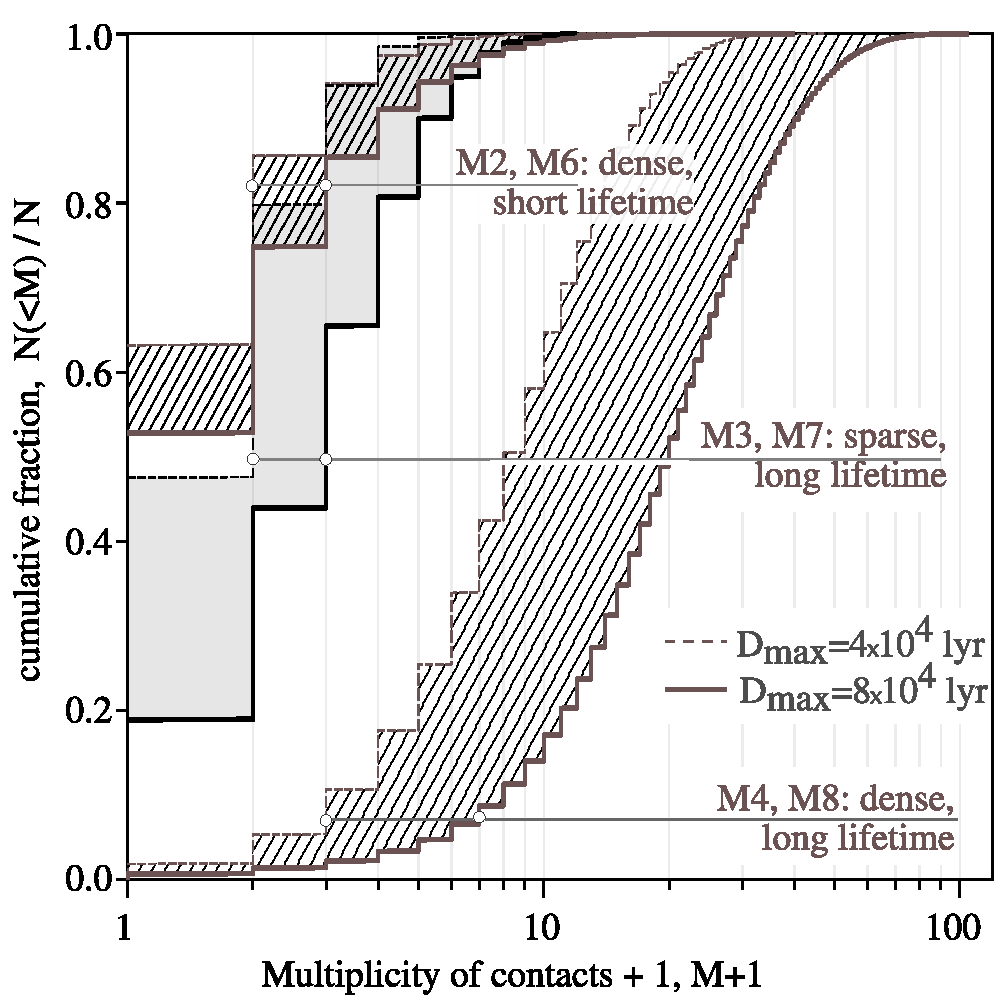
\includegraphics[width=0.5\textwidth]{F_number_of_contacts.pdf}
   \caption{
   %
Empirical cumulative distributions of the number contacts
for \cetis in four different samples (M5, M6, M7, M8) with two
values for the range of the signal reach: D$_{\rm max}$=40000 ly (blue),  and 
D$_{\rm max}$=80000 ly (orange).
%
Except for the models corresponding to a densely populated galaxy with
long--living \cetis, the \cetis which receive more than 10 contacts
are very unlikely.
%
See Table \ref{T_selected_models} for model descriptions.
%
   } \label{F_number_of_contacts}
\end{figure}
        
 

\subsection{Complexity of the model}
%{{{



In this Section we discuss the degree of complexity in the model, considering a compromise between the accuracy of the
model and the number of parameters that are free or with a high uncertainty.
%
Firstly, we emphasise that the odds of a causal contact between two \cetis{} should not be considered as the odds of a
contact between two intelligent civilisations, and in fact the latter could be much lesser than the former.
%
Indeed, in order to establish a contact between any two entities, a minimum degree of compatibility must be accomplished
without any previous agreement, making the possibility of a contact with a message that could be deciphered highly rare
\citep[see e.g. ][]{forgan_collimated_2014}.
%
Besides the trade--off between the simplicity and the complexity of the experiments, further analysis could be performed
following this framework in order to explore possible implications of the results for more detailed configurations.
%
For example, the communication method (isotropic, collimated, serendipitous) can affect the observables, making it
necessary to implement a correction factor.
%
Taking this into account, our results regarding the probability of causal contact should be considered as upper limits
for effective contacts, since they depend on the efficiency of both the emitter and the receiver to broadcast and scan
the sky for intelligent signals, respectively \citep{grimaldi_signal_2017}.
%
A correction by coverage ratio in the detection and by a targeting ratio in the emission could be easily implemented in
the simulation, although the effect of reducing the probability of contact is basically the product of the efficiency
ratios and thus such implementation is not necessary.
%
Therefore, the values of the probabilities could be modified by a constant correction factor equal to the combined
emission/reception efficiency \citep{smith_broadcasting_2009, anchordoqui_upper_2019, forgan_collimated_2014} or for
beam-like transmissions \citep{grimaldi_signal_2017}. 
%
Other considerations include the effects of alignments, the use of stars as sources or amplifiers \citep{Edmondson2003,
borra_searching_2012}, the nature of the message carrier.
%
Another improvement could be the use of a spatial distribution that resembles the spiral shape and the width of the disc
of the Galaxy.
%
Regarding the distributions of the parameters, different distribution functions for the mean lifetime of \cetis{} can be
implemented as alternatives.
%
Finally, regarding the degree of idealisation, the model admits different efficiencies for the sphere of the causal
region of each \ceti{}, featuring different searching strategies \citep{hippke_interstellar_2017}. 
%
It is also possible to consider that $D_{\rm max}$ is different for different \cetis{}.
%
For example, a power law where powerful emissions are rare and low emissions are common could be an improvement to the
model.
%
In this work we chose not to implement this for the sake of simplicity.
%
Finally, the role of the message contents could influence on the lifespan of a \ceti{} that receives a message, although
the implementation of such behaviour would increase the number of free parameters and would be more speculative.     

%}}}
     



\subsection{Discrete event process}
%{{{

A discrete event simulation is performed for a given model $M(\tau_a,
\tau_s, D_{\rm max})$ by keeping track of a set of variables that change each time an event happens. 
%
In addition, the model comprises elements that are fixed for all simulations, for example, the functional forms of the statistical distributions and the adopted values of particular variables (see Table XXX).
%
The main variables that follow the evolution of the simulation are: the positions of stars, which are sampled randomly within the GHZ; the time of the awakening of each \ceti{} (A event); and the time of the vanishing of each \ceti{} (D event). 
%
The variables that can be deduced from the previous ones include: the number of \cetis{} in casual contact with at least another \ceti{} at a given time; the number of \cetis{} as a function of time; the number of \cetis{} that receive a message at least one time; the number of \cetis{} that receive a message at least one time and successfully deliver an answer; and the number distribution of waiting time to receive a message.
%
All these quantities are updated each time one of the four events (A, B, C, D) occurs.   





          
%%% comparar con el stochsatic cellular automata
% ver libro Solving Fermi paradox, sec. 27.3.1

%}}}
           
  
\begin{figure*} % 2D color plot
   \centering
   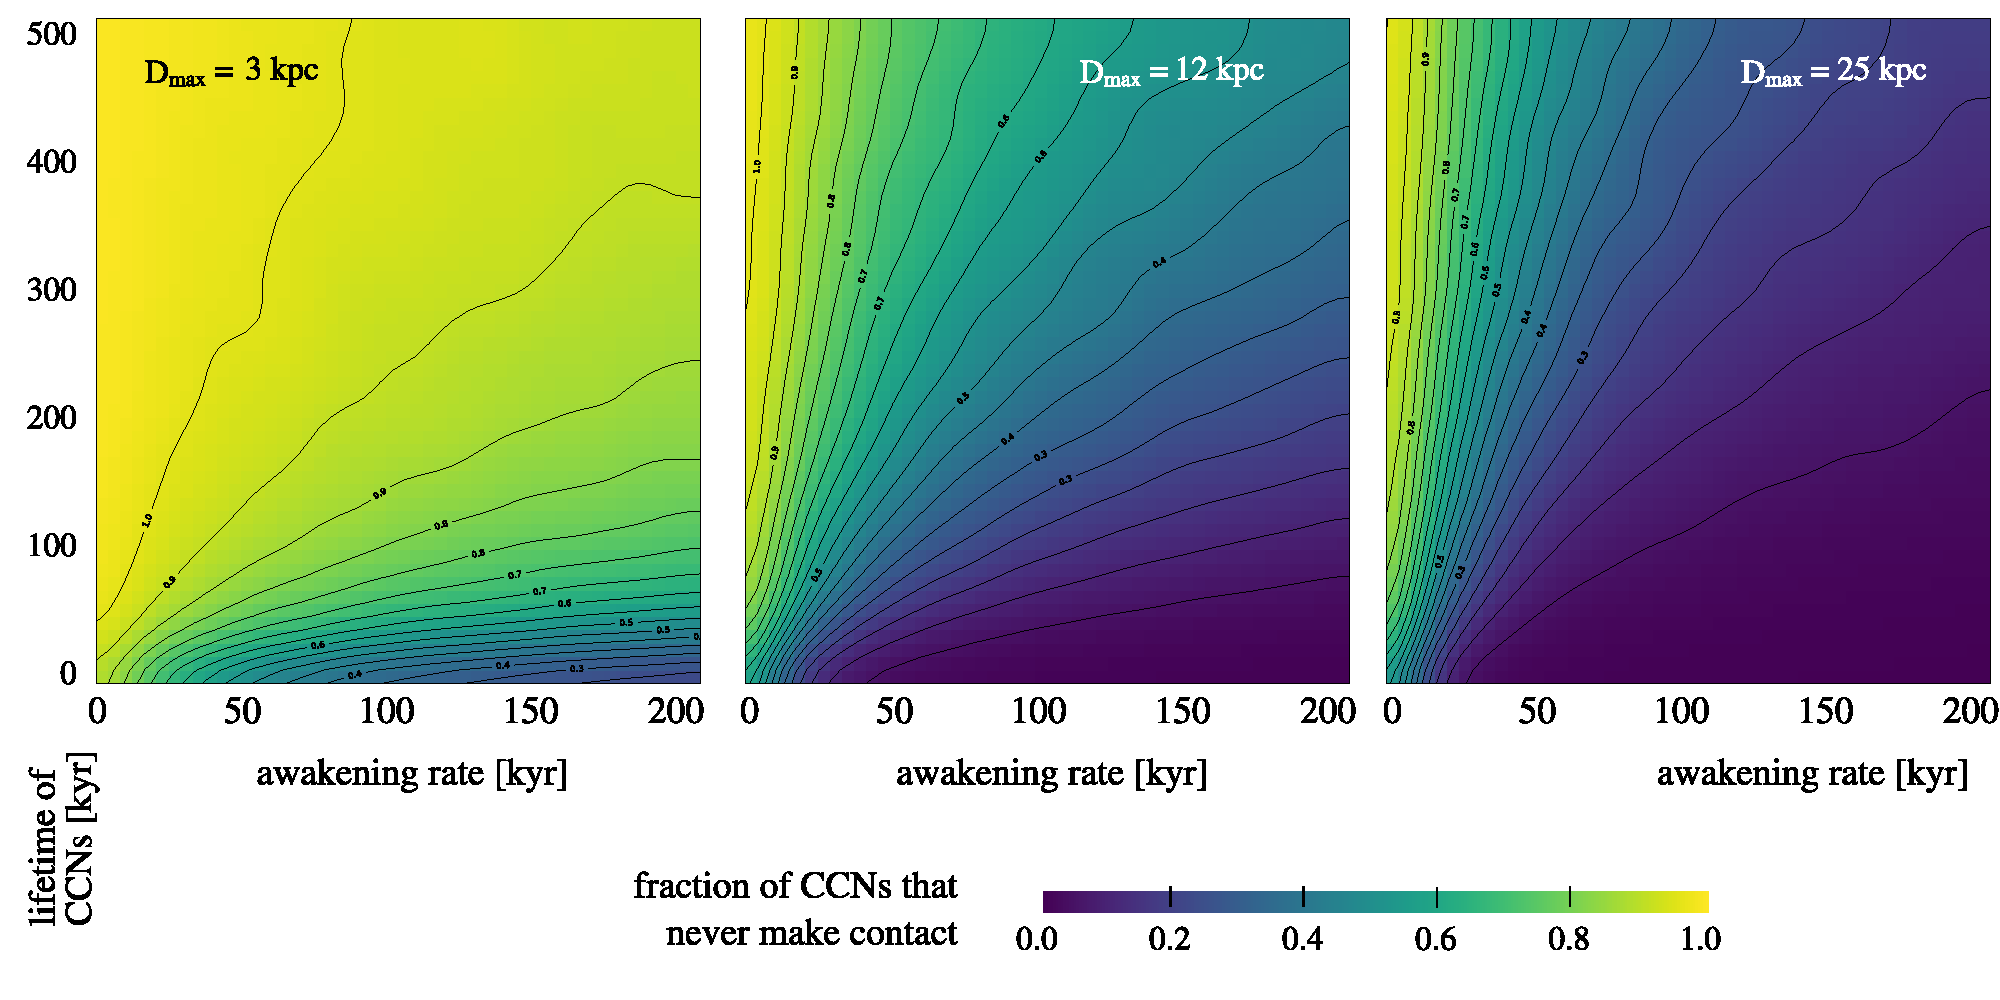
\includegraphics[width=\textwidth]{F_never_contact.pdf}
   \caption{
   %
Rate of MPLs that never make contact (listening) as a
function of $\tau_a$ and $\tau_s$, for 
$D_{\rm max}$=10000 (left panel),
$D_{\rm max}$=40000 (middle panel), and
$D_{\rm max}$=80000 (right panel)
%
   }
   \label{F_never_contact}
\end{figure*}
 
\begin{figure*} % 2D color plot
   \centering
   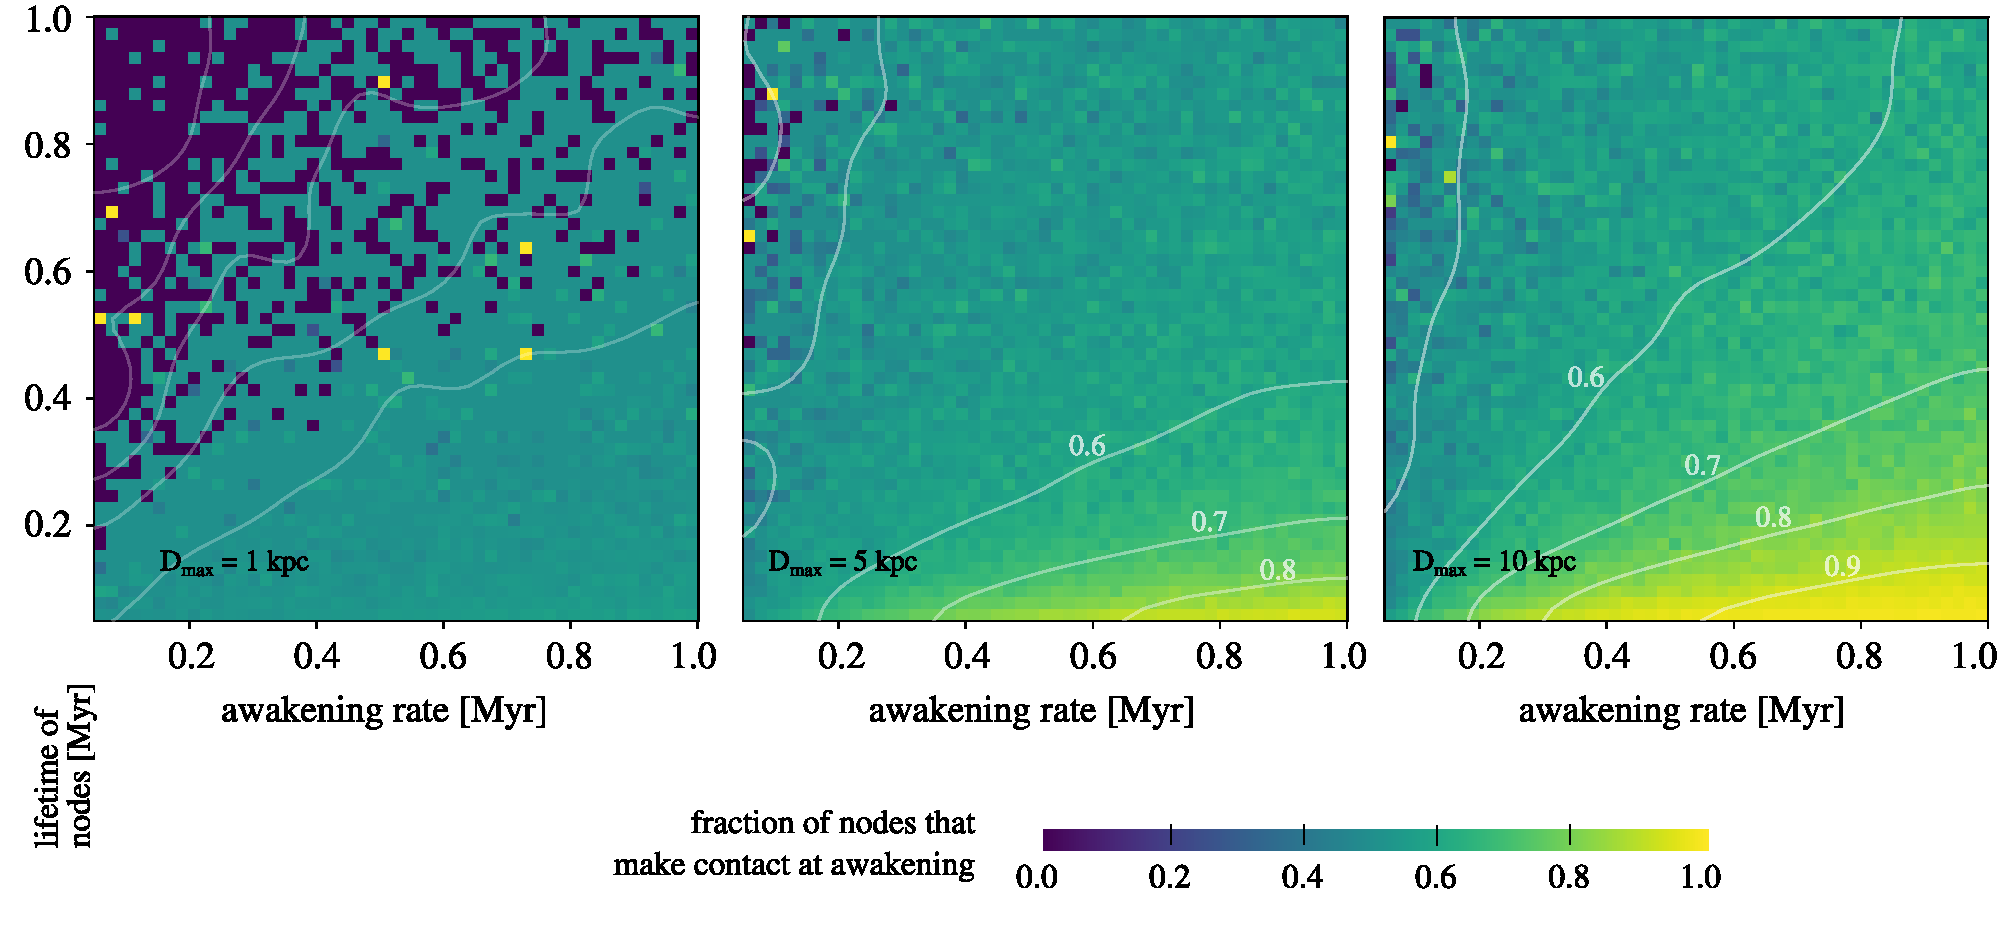
\includegraphics[width=\textwidth]{F_C_at_A.pdf}
   \caption{
   %
Rate of MPLs that listen at the moment of the
awakening, as a funcion of $\tau_a$ and $\tau_s$, for
$D_{\rm max}$=10000 (left panel),
$D_{\rm max}$=40000 (middle panel), and
$D_{\rm max}$=80000 (right panel)
%
   }
   \label{F_C_at_A}
\end{figure*}
        

                     

\subsection{Model for \cetis{}}
%{{{

Since the method is based on events, the first step is to define the relationships between them and how events trigger changes on the state of the system.
%
Once an event is produced, the system is updated by saving the corresponding change in the related variables.
%
For example, a B-type event diminishes the number of active \cetis{} by one, and also could affect the number of ongoing communications.
%
We consider a first approach to the galactic habitable zone as a 2-dimensional annular region.
%
The adopted values for the geometry of the GHZ are 2 kpc and 8 kpc, for the inner and outer radius, respectively \citep{lineweaver_galactic_2004}. 
% ojo, ese paper dice 7-9 kpc, o sea tiene un limite superior mucho
% mas chico...
%
This simple model does not take into account the variations in stellar density given by the spiral structure of the Galaxy.
%
The main task in setting a DE simulation is to define the events and what changes do these events produce on the system.
%
Although there are several possible approaches, we chose to follow the evolution of the system according to the following events:

\begin{enumerate}
   \item[(A)] Awakening: A new \ceti{} acquires the ability to emit
      and receive messages and starts to actively broadcast and
      lookout for messages.
   \item[(C)] Contact: A new one-way causal contact is established
      (does not require the awareness of the involved \cetis{}.)
   \item[(B)] Blackout: An existing causal contact is interrupted,
      with or without the occurrence of a doomsday event.
   \item[(D)] Doomsday: An old \ceti{} disappears, or halts its
      communication activities.
\end{enumerate}

We have chosen this nomenclature so that it can be easily remembered
from the initials A, B, C, D.
%
The \blackout is produced when one of the two \cetis{} halts in its
capability of emitting and receiving signals.
%
It can occur at the same time the \doomsday or before.
%
Similarly, a \ccontact can be produced at the time of the \aawakening
or later, and there can be several \contacts for the same node.
%
The time marks for each event (A and D for each \ceti{} and C and B
for each causal contact) are stored as a result of the simulation.
%
Also, the list of active \cetis{} is obtained as a function of time.
%
%Some fixed variables must be set in order to carry out the simulation:
%the size of the Galactic Habitable Zone, the mean lifetime of a
%\ceti{}, $\tau_s$, the mean waiting time for the appearance of another
%\ceti{}, $\tau_a$, and the maximum distance a message can be detected.



% The Galactic Habitable Zone is set at fixed values of the inner and outer
% radii, radial symmetry is assumed, and the with of the galactic disk
% is neglected compared to the radial size.
% %
% The two radii are measured in light years, with the aim to maintain a
% single and comprehensive unit for both space and time coordinates. 
%
%}}}


\subsection{Model implementation}
%{{{


% hearsay 
%
In order to make a reproducible project, we developed the tools
that allow to run and obtain the results shown in this work.
%
The simulations were implemented on a Python-3 code, dubbed \hs{},
which is publicly accessible through the GitHub
platform\footnote{https://github.com/mlares/hearsay} under the
MIT-license.
%
The project is in the process of registration with the ‘’Astrophysics
Source Code Library’’ \citep[ASCL, ][]{2015JORS....3E..15A,
2020ASPC..522..731A}
%
In order to achieve high performance we made use of vectorised methods
and array broadcasting properties provided by the NumPy package
\citep{oliphant_numpy_2006, vanderwalt_numpy_2011}
%
The combination of C-compiled Numpy routines for numerical
computations with a high-level language allows to obtain an easily
comprehensible and maintainable code.
%
From the viewpoint of a user, \hs{} is an object-oriented package that
exposes the main functionalities as classes and methods.
%
In the configuration step, the user prepares the set of simulation
parameters through an initialisation file.
%
Since configuration files and simulation results are persistent, it is
straightforward to keep track of different experiments and the
experiments can be revisited easily.
%
An in-depth description of the methods can be found in the
documentation, which is automatically generated from \hs{} docstrings
and made public in the read-the-docs service.



%Quality assurance
%
Regarding the quality assurance of the software, we endorse the PEP-8
style guide for python (van Rossum et al. 2001) throughout the entire
project, which improves the code maintainability and helps to minimise
the so called ''code-entropy'' of future versions.
%
The deviations in style were analysed with the flake8 tool, which
improves the readability and consistency of the code.
%
Testing and code coverage have been applied to the package and the
development process as standard qualitative and quantitative metrics.
%
The different parts and functions can be validated to assert if they
return the expected results on specific test cases and testing
scenarios \citep{jazayeri_engeneering_2007}.
%
On the other hand, code coverage measures the fraction visited and
executed in the code by the testing procedure
\citep{miller_testing_1963}.
%
The advantage of an exhaustive code-coverage is that it ensures that
most of the sources of errors have been considered.
%
In the \hs{} project we provide test tools for the distinct parts of
the simulation setup and run, reaching a 99\% of code coverage in the
version used for this work.
%
For every new version of the code, all these quality assurance methods
and metrics are run automatically by a continuous-integration service.
%
It is possible to reproduce the experiments performed in this work
using the \hs{} package.
%
The installation is available through a git repository and also on the
Python Package Index (PyPI).
%
Since the simulation setup is configurable, the time required for a
simulation to complete depends on the simulation parameters.
%
It also depends on the hardware that is used to make the run, and on whether the parallel option is set.
%
However, it is simple to make a local run of limited versions of the experiments to have a sense of the time required by
the code to complete the simulations.
%
More information on this can be found on the documentation of the software, available at
\url{https://hearsay.readthedocs.io/en/latest/}.

%}}}


\begin{figure}
   \centering
   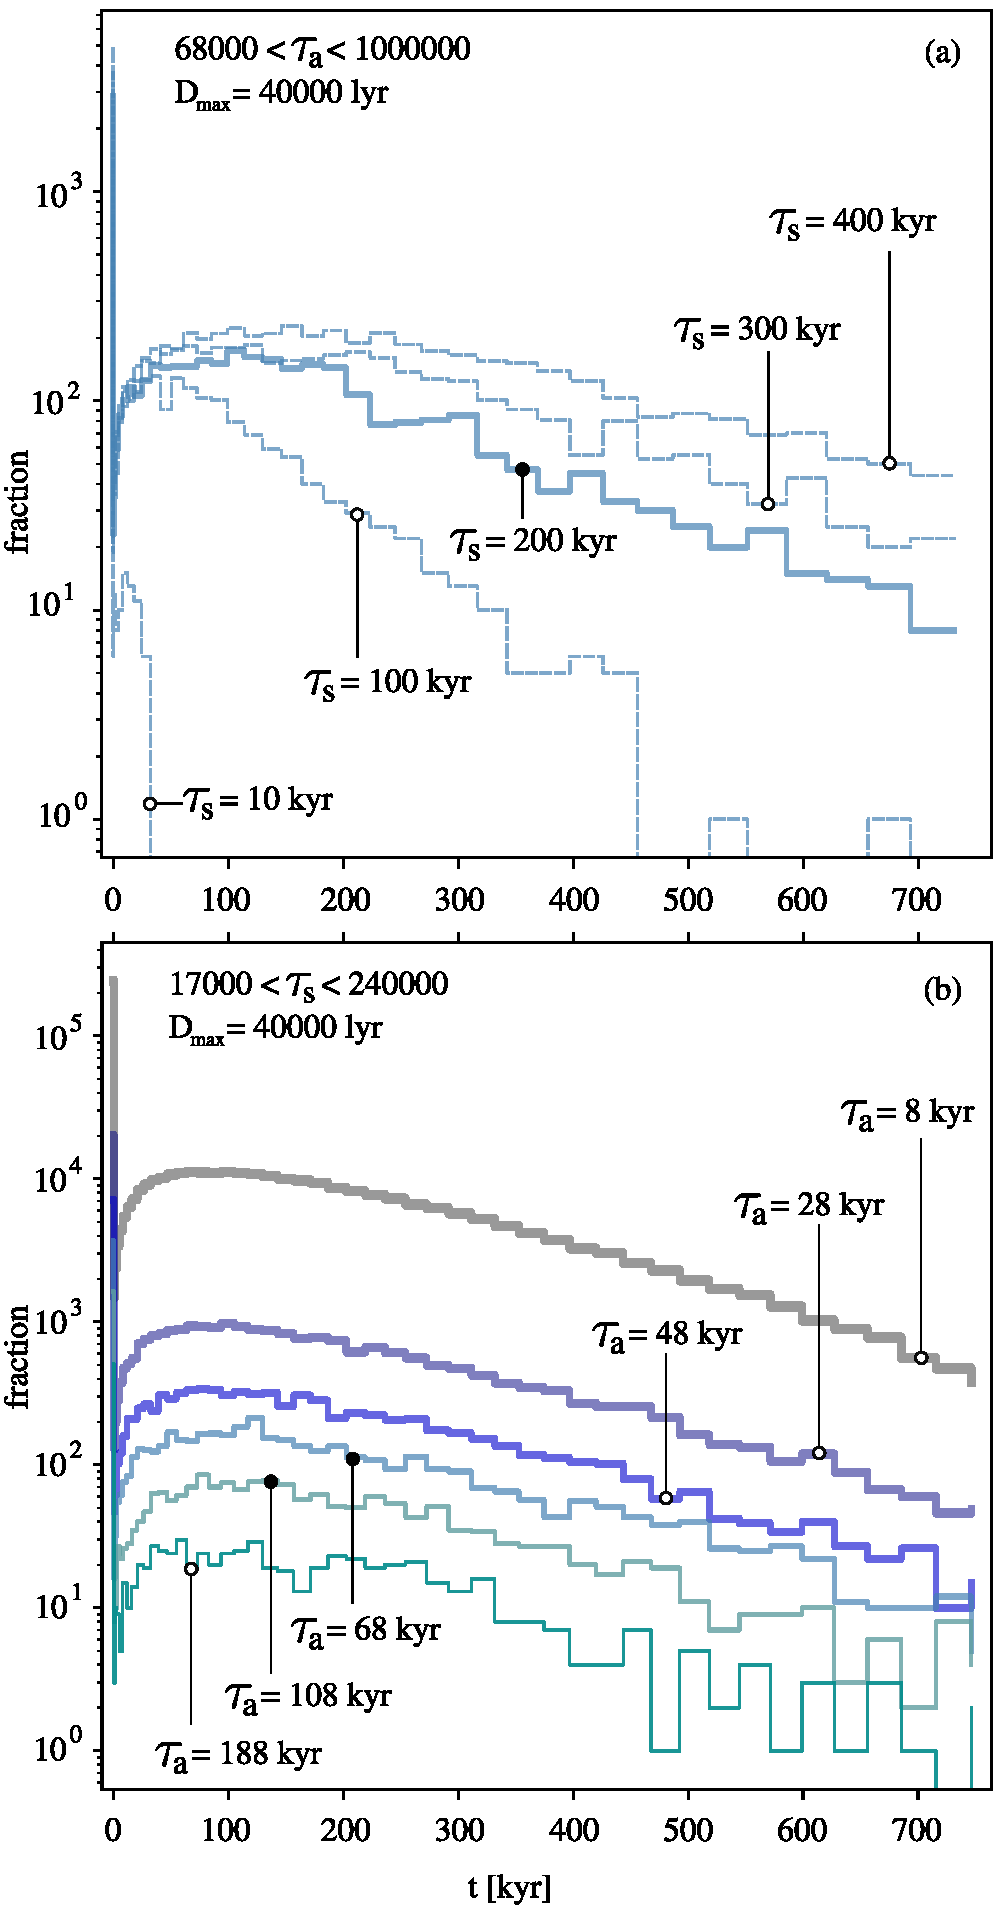
\includegraphics[width=0.5\textwidth]{F_waiting_for_1C.pdf}
   \caption{
   %
Histograms of the mean waiting times for the first contact, for
several models.
%
Left panel shows the histograms for several values of $\tau_a$, and
$\tau_s$ in the range 17000-24000 yr.
%
Right panel shows the histograms for several values of $\tau_s$, and
$\tau_a$ in the range 68000-100000 yr.
%
The shape of the histograms does not change when $\tau_a$ is
modified, but significantly changes when $\tau_s$ is modified. 
%
   }
   \label{F_waiting_for_1C}
\end{figure}

\setlength{\tabcolsep}{10pt}
\begin{table*}
\centering
\begin{tabular}{ccccc}
\hline
   Model subset & D$_{\rm max}$ [lyr] & $\tau_a$ interval [yr] & $\tau_s$ interval 
   [yr]& description  \\
\hline
M1 & 40000 & [10000, 30000]   & [10000, 50000]   &dense, short lifetime\\
M2 & 40000 & [170000, 190000] & [10000, 50000]   &sparse, short lifetime\\
M3 & 40000 & [10000, 30000]   & [400000, 440000] &dense, long lifetime \\
M4 & 40000 & [170000, 190000] & [400000, 440000] &sparse, long lifetime\\
%
M5 & 80000 & [10000, 30000]   & [10000, 50000]   &dense, short lifetime\\
M6 & 80000 & [170000, 190000] & [10000, 50000]   &sparse, short lifetime\\
M7 & 80000 & [10000, 30000]   & [400000, 440000] &dense, long lifetime \\
M8 & 80000 & [170000, 190000] & [400000, 440000] &sparse, long lifetime\\
%
\hline
\end{tabular}
\caption{Selected models to analyze the behavior of simulation outputs
   and their dependence on simulation parameters.}
\label{T_selected_models}
\end{table*}

 


%%% S E C T I O N - - - - - - - - - - - - - - - - - - - - - - -
\section{Results: exploring the parameter space}\label{S_results}
%{{{

We implemented the simulation of a regular grid of models varying over
the hypothesis space, which covers 15000 different models.
%
For each model, we simulated 50 realizations with different random
seeds, in order to perform a MonteCarlo estimation of the variance.
%
The parameters for the temporal aspects of the simulation (the mean
waiting time for the next awakening, $\left<\tau_a\right>$, and the
mean lifetime, $\left<\tau_s\right>$) cover the ranges 10$^2$-10$^6$
yr, with a linear partition of 50 values for each parameter.
%
For the D$_{\rm max}$ parameter, we take the range 30~pc to 10~kpc, on
50 linear bins.
%
This setup makes a total of 750000 simulations, each covering a time
range of ten million years.
%
\ttn{1}
%
In the Table \ref{T_simu_hypotheses} we show the three variable
parameters, the ranges of their values and the number of bins that
have been explored in the numerical experiments.
%
We also show the set of fixed parameters that take part in the simulation,
their values and the hypotheses that they represent.




As a product of the simulations, several quantities can be obtained.
%
Some of them are directly derived from the discrete events, namely,
the ID of emitting and receiving \cetis{} and the position in the
galaxy.
%
We also save the times of each of the events that are relevant to keep
track of the number of \cetis{} for each simulation, i.e., the times
of the four types of events.
%
the times of C-type and B-type events are used to derive the number of
contacts.
%
We also obtain quantities that represent the
properties of the \cetis{}, for example the total time elapsed between the
A-type and the D-type of each node, which represent the corresponding
lifetimes of the nodes.
%
The time span of a \ceti{} listening another or being listened by another
can also be derived by keepig track of the times of the events in a simulation.
%
This way we can also compute the distribution in the galaxy of
\cetis{}
that reach contact, the distributions of the waiting times until the 
first contact or the distributions of
waiting times until the next contact.
%
The following properties of the population of \cetis{} can be derived:
%
the fraction of the lifetime a node is listening
to
at least another node (i.e., in their causal cone),
%
the age of
contacted \cetis{} at first contact,
%
the fraction of \cetis{} where the first contact is
given at the awakening,
%
the distribution of the number of contacts for
each \ceti{},
%
the distribution of the number of contacts as a function of
the age of the node,
%
the number of contacts as a function of time in the galaxy,
%
the fractions of nodes that succeed in making contact,
%
and the distribution of
distances between contacted nodes.
%
Another useful derived quantity is the duration of two-way
communication channels or the fraction of contacts that admit a
response.
% 
It is also possible to analyze the relations between the distance to
\ceti{} vs. the time of two-way communications, the distance to \ceti{} vs. the
age of contacted node, the age of a node and the maximum number of
contacted nodes before the D--type event, or the lifespan of a node vs. the
maximum number of contacts.
%
All these quantities can be analyzed as a function of the
simulation parameters.
%
We chose eight models that are on opposed regions of the
explored parameter space, and cover
all possible combinations of 
short/long lifetimes, short/long
waiting times for the next \ceti{} to appear in the galaxy and short/large
range reach of the signal.
%
\ttn{2}
%
The details of each model are summarized in the
Table~\ref{T_selected_models}.

%}}}


\subsection{Membership to the network of connected \cetis{}}\label{SS_members}
%{{{

\ffn{3}
%
In Fig.~\ref{F_number_of_contacts} we show the empirical cumulative
distributions of the number contacts for \cetis{} in six different
samples, including short and long lifetimes
$\left(\,\left<\tau_s\right>=\right.$10000~yr and
$\left<\tau_s\right>$=100000~yr, respectively$\left.\right)$, dense
and sparse spatial distribution
$\left(\,\left<\tau_a\right>=\right.$10000~yr and
$\left<\tau_a\right>$= 100000~yr, respectively$\left.\right)$, and two
different signal reach ranges (D$_{\rm max}$=40000 lyr and
D$_{\rm max}$=80000~lyr).
%
The models M1 and M5 are not shown, since in both cases the total
number of contacts is different from zero for less than the five per
cent of the \cetis{}.
%
The areas between models with the same mean lifetime and mean
awakening time are shaded for visualization purposes.
%
As it can be seen from this Figure, the mean lifetime is more
determinant than the mean awakening rate (dense and sparse,
represented by a different shade) for the number of contacts.
%
As expected, of the samples with the longest $D_{\rm max}$ the model with
a dense awakening in the timeline (low $\left<\tau_a\right>$) and a
long lifetime (high $\left<\tau_s\right>$), is the model that
maximizes the number of contacts, reaching a maximum of order 20
contacts for a single \ceti{}.
%
Similarly, for the models with long signal range
($D_{\rm max}=80000\,lyr$), the one which is dense and with long lifetime
has the maximum number of contacts, reaching nearly 100 contacts for
each \ceti{} in its entire lifetime.
%
This is considerably larger than any model with a shorter lifetime,
which produce a number of contacts of at most the order of ten
contacts per \ceti{}.
%
A couple of comments are worth to mention about this plot, namely, it
has a logarithmic scale on the x-axis, and it is the cumulative, not
differential, empirical distribution, so that the differences in the
number of contacts for different models are relatively large.
%
Another interesting feature observed in this Figure, is that for the
models analyzed, there are \cetis{} that have no causal contacts with
any other \ceti{} during their whole lifetime.
%
The fraction of \cetis{} with no contact ranges from nearly 20\% up to
nearly 90\% (models M1 and M5, not shown), except for the dense and
long lifetime models, for which almost all \cetis{} make at least one
contact.
%
Since these results depend on just eight models, we analyze the
properties of the frequency of contacts as a function of both the mean
lifetime and the mean awakening time.
%
\ffn{4}
%
On Fig.~\ref{F_never_contact} we show 2D color maps with the fraction
of \cetis{} in the simulations that never make contact (i.e., never
listen to another \ceti{}), as a function of the mean lifetime
($\left<\tau_s\right>$, in the range 0--500 yr) and the mean awakening
time ($\left<\tau_a\right>$, in the range 0--200 yr), for three
different values of the maximum signal range, $D_{\rm max}=10000$~yr (left
panel), $D_{\rm max}=40000$~yr (middle panel), and $D_{\rm max}=80000$~yr
(right panel).
%
A clear pattern emerges in this Figure, showing that the probability
for a \ceti{} of making causal contact with at least another \ceti{}
during their entire lifetime, increases with increasing $D_{\rm max}$,
increasing $\left<\tau_s\right>$ and decreasing $\left<\tau_a\right>$,
following a roughly linear dependence with the three parameters.


The number of \cetis{} that do not succeed in reaching the
causal contact regions of other nodes is a useful indicator of
the
degree of isolation.
%
On the other hand, there is also the chance that a number of
\cetis{} are already in the causal contact region of other nodes,
at the time of their A-type events.
%
\ffn{5}
%
The fraction of \cetis{} that make the first contact at the awakening
event is shown in the Fig.~\ref{F_C_at_A}, 
as a function of the mean lifetime
($\left<\tau_s\right>$, in the range 0--500 yr) and the mean awakening
time ($\left<\tau_a\right>$, in the range 0--200 yr).
%
The three panels correspond to different values of the maximum signal
range ($D_{\rm max}$),
as indicated in the Figure:
%
$D_{\rm max}=10000$~yr (left
panel), $D_{\rm max}=40000$~yr (middle panel), and $D_{\rm max}=80000$~yr
(right panel).
%
These probabilities are consistent with the ones on the previous
Figure.
%
Although they are not complementary, it is clear that the dependence
with the three parameters is roughly linear in both cases.
%
%% DISCUTIR ESTOS RESUOLTADOS SEGUN LA LITERATURA


%

%}}}

\subsection{Waiting time for a first contact}\label{SS_waiting}
%{{{

In this subsection we analyze the distribution of the waiting times for
a first contact.
%
Such distribution can be considered to compute the probability for a
random \ceti{} to carry out a SETI project and spend a given time until
the first contact is made, under the hypotheses of the experiment.
%
\ffn{6}
%
In the Fig.~\ref{F_waiting_for_1C} we show the histograms of the mean
waiting times for the first contact, for several models.
%
Upper panel (a) panel shows the histograms for several values of the
mean survival time $\tau_s$, with the mean awakening time $\tau_a$ in
the range 68000-100000 yr.
%
Lower panel (b) shows the histograms for several values of $\tau_a$,
with $\tau_s$ in the range 17000-24000 yr.
%
As it can be seen, the shape of the histograms is almost the same when
$\tau_a$ is modified (panel (b)), but significantly changes when
$\tau_s$ is modified (panel (a)). 
%
For different values of $\tau_a$, the shape of the distribution is
similar, and the main difference is given by the variation on the number of
contacts on the different models.
%
Conversely, for different values of $\tau_s$ (at a fixed range for
$\tau_a$), the shape of the
distribution varies significantly.

 

The fraction of the \cetis{} that have made at least one contact, as a
function of the elapsed time since the awakening, is computed with
respect to the total number of nodes that make causal contact at least
one time in the time range from the A--type up to the D--type
events.
%
From a frequentist approach, the cumulative fraction of contacts
from the awakening
($t=$0~yr) up to a given time are related to the estimation of the
probability of listening during that time interval and reaching to
causal contact region of at least another node.
%
The complement of this value is the probability of observing in a time
interval with no success, i.e., without ever happening a C--type
event.
%
Clearly, this probability diminishes with time and tends to zero for
large time periods, meaning the a \ceti{} will eventually get aware of
the presence of other \cetis{}


Remarkably, the differential probability of making a causal contact reach its
maximum at the awakening event for all models.
%
That is, for a short period of time the initial moment is the most promising
for making a (causal) contact, for a given technology.
%
This allows to consider the fact that for the nearly 50 years SETI
programs have been active, no contact event has been reported.
%
This offers a new approach to SETI programs, where the
search for new communication technologies or the exploration of
new communication channels has a fundamental role.
%
Moreover, as it can be seen in the Fig.~\ref{F_waiting_for_1C}, there
is a maximum probability of making the first causal contact at nearly
100000 years.
%
The probability of such a contact does not grows linearly
with the observing time, but is greater during the first 100
millennia.

%}}}


%%% S E C T I O N - - - - - - - - - - - - - - - - - - - - - - -
\section{Discussion}\label{S_discussion}
%{{{


We have implemented a suite of simulations, following a stochastic approach, to explore a three dimensional hypothesis space of a simple model that accounts for the causal connections between communicating civilisations in the Galaxy. The different models can be generated with a minimal number of assumptions. We argue that three parameters can describe a variety of situations, ranging from a galaxy model where an intelligent civilization is very rare, to a galaxy model populated with plenty of civilisations in causal contact. With this approach, we can estimate several quantities as a function of the parameters on the hypothesis space, so we explored the outcomes of different models that can be derived from the simulations. For instance, it is possible to estimate the timescale for an uninterrupted SETI-equivalent effort to reach success, in terms of different model parameters that reflect different, so far unknown, scenarios for the appearance of intelligent life on the Galaxy.



Although the simulations use a number of speculative assumptions, we
argue that the limited knowledge about the origin and persistence of
life in the Galaxy does not worth the implementation of more detailed
or sophisticated models.
%
Instead, we take advantage of the simplicity of the model to explore
the hypothesis space, i.e., the three--dimensional parameter space of
the parametric model, in order to gain insight on the consequences of
different scenarios for the search of intelligent life.
%
Our analysis is not centered in obtaining the odds for the Earth
to make contact with another intelligent civilization.
%
Instead, we focus on obtaining a statistical, parameter dependent
description of the possible properties of the communication networks
that comprise sets of nodes with broadcasting and reception
capabilities.
%
This causally connected nodes are sparsely distributed in both space
and time, making analytical treatments difficult and justifying
the simulation approach.


Under the hypotheses of our experiments, we conclude that a causal
contact is extremely unlikely unless the galaxy is densely populated
by intelligent civilizations with large average lifetimes.
%
On average, in order to have at least one contact in the entire lifetime
of the \ceti{}, there must appear a mean of at least one \ceti{}
every $\sim$20000 yr, with a mean active period of at least
$\sim$30000 yr.
%
This result is qualitatively similar to the results presented by
several authors, which state that a contact between the Earth and
another intelligent civilization in the Galaxy is quite unlikely,
provided the maximum distance of the signal and the lifetime of the
emitter are not large enough.
%
This analysis supports the idea that, in order to increase the
possibilities of a contact, more active strategies of the emitter
would be required.
%
Some proposals in this direction include intertellar exploration,
colonization and settlement \citep{brin_great_1983, Dosovic2019,
galera_invasion_2019}, although it would require large temporal
scales.
%
\citet{Dosovic2019} use probabilistic cellular automaton simulations
to explore the parameter space of a model with colonization and
catastrophic events.
%
According to the timescales involved, the results could explain the
Fermi paradox.
%
Although our work does not take into account the colonization
hypothesis, it does consider catastrophic events implicitly in the
mean value and distribution of the lifetime, $\left<\tau_s\right>$.
%
Other strategies could also increase the probability of contacts, for
example panspermia \citep[e.g.,][]{starling_virulence_2013} or
self--replicating probes \citep[e.g.,][]{barlow_galactic_2013},
although they would be too slow to make a significant impact on the
communication network among intelligent civilizations.
%
Our results are also consistent with those presented by
\citet{grimaldi_signal_2017}, who estimate an upper bound for the mean
number of extraterrestrial civilizations that could contact Earth
using Monte Carlo simulations, from a statistical model where the width
of the Galactic disk is not negligible.
%
On the other hand, taking into account the probability of contact with
radio signals not sent intentionally \citep{horvat_calculating_2007},
our analysis would imply a highly populated solar neighborhood.
%
Unlike most 
of the studies that make use of statistical models or
simulations \citep{cirkovic_temporal_2004, smith_broadcasting_2009,
bloetscher_using_2019}, our approach does not relay on the Drake
equation.
%
Thus, it does not need
a detailed description or modeling of physical processes that give rise to
intelligent life.
%
However, we argue that it is a valid empirical formulation to discuss
the probabilities of contact, and the time scales involed in the
problem.
%
Ours is an alternative to the method proposed by
\citet{balbi_impact_2018}, who perform an analysis based on the Earth
and use a different model, although our results agree in general.

We also fond that there 
is a balance between the density of \cetis{} and the mean
lifetime since, as expected, a lower density can be compensated by a
longer active time period.
%
However, a large number of nodes does not easily compensate their
short lives to reach the same probability of causal contact than in
the case of a less populated galaxy but with very ancient
civilizations.
%
In all cases, for a short period of time (for instance, the time SETI
programs have been active on Earth), the maximum probability of making
a contact occurs at the moment of the awakening.
%
This suggests the possibility that an alternative SETI strategy could
be the search for alternative message carriers, for the case in which
the search has not been performed on the adequate channels.
%
Then, if a contact is produced for the first time, the origin of the
signal is more likely to be very old.
%
Also, the chances of entering the causal connected zone of a \ceti{}
does not grow linearly, but favours the first period of 100000 years.


In the approach of this work, we have used computer simulations to address
the problem of the probabilities of causal contacts between locations
in the galaxy with the possibility of sending and receiving messages.
%
Instead of making a number of assumptions, we have explored the
hypothesis space, reducing the problem to only three parameters and a
few simple hypothesis to perform a complete model for the population and
communication network in the galaxy.
%
This allows to consider the Fermi paradox from a new perspective, and
to propose an alternative treatment for the number of intelligent
emitter/receivers.
%
The short time interval between the
rise and fall of civilizations, compared to the age and extension of
our Galaxy, is a fundamental limitation for the number of contacts.
%
Thus, the temporal dimension, which is missing in the Drake
equation, is a key factor to understand the network of contacts on
different scenarios.

%}}}

\ack[Acknowledgement]{
%
This work was partially supported by the Consejo Nacional de
Investigaciones Cient\'{\i}ficas y T\'ecnicas (CONICET, Argentina),
the Secretar\'{\i}a de Ciencia y Tecnolog\'{\i}a, Universidad Nacional
de C\'ordoba, Argentina, and the Universidad Cat\'olica de C\'ordoba,
Argentina.
%
This research has made use of NASA's Astrophysics Data System.
%
Plots and simulations were made with software developed by the authors
using R and python languages. Plots were postprocessed with inkscape.
%
}

\ack[Disclosure statement]{
%
No competing financial interests exist.
%
}

\bibliographystyle{mn2e}
\setlength{\bibsep}{0.0pt}
\bibliography{biblio_seti, biblio_software}

\end{document}
